
\subsection{Darcy and Burgers Equations}
\label{ssec:darcyburgers}

\done{Is $s$ defined anywhere (see Tables); even if it is recall
its definition in the table captions?}

\postponed{These Darcy and Burgers results show FNO is the best but
in what sense are they "fair" comparisons? Are the other methods
using same number of parameters; same amount of training time;
same ammount of evaluation time? This discussion needs to be
sharper.}


In the following section, we compare four methods presented in this paper, with different operator approximation benchmarks; we study the Darcy flow problem introduced in Subsection~\ref{ssec:darcy} and the Burgers' equation problem introduced in Subsection~\ref{ssec:burgers}. The solution operators of interest are defined by \eqref{eq:darcysolutionop}
and \eqref{eq:burgerssolutionop}. We use the following abbreviations for the methods against which we benchmark.

\begin{itemize}
    \item {\bf NN} is a standard point-wise feedforward neural network. It is mesh-free, but performs badly due to lack of neighbor information. We use standard fully connected neural networks with 8 layers and width 1000.
    \item {\bf FCN} is the state of the art neural network method based on Fully Convolution Network \citep{Zabaras}. It has a dominating performance for small grids $s=61$. But fully convolution networks are mesh-dependent and therefore their error grows when moving to a larger grid.
    \item {\bf PCA+NN} is an instantiation of the methodology proposed in \cite{Kovachki}: using PCA as an autoencoder on both the input and output spaces and interpolating the latent spaces with a standard fully connected neural network with width 200. The method provably obtains mesh-independent error and can learn purely from data, however the solution can only be evaluated on the same mesh as the training data.  
    \item {\bf RBM} is the classical Reduced Basis Method (using a PCA basis), which is widely used in applications and provably obtains mesh-independent error \citep{DeVoreReducedBasis}. This method has good performance, but the solutions can only be evaluated on the same mesh as the training data and one needs knowledge of the PDE to employ it.
    \item {\bf DeepONet} is the Deep Operator network \citep{lu2019deeponet} that comes equipped with an approximation theory \citep{lanthaler2021error}. We use the unstacked version with width 200 which is precisely defined in the original work \citep{lu2019deeponet}. We use standard fully connected neural networks with 8 layers and width 200. 
\end{itemize}

\begin{figure}
    \centering
    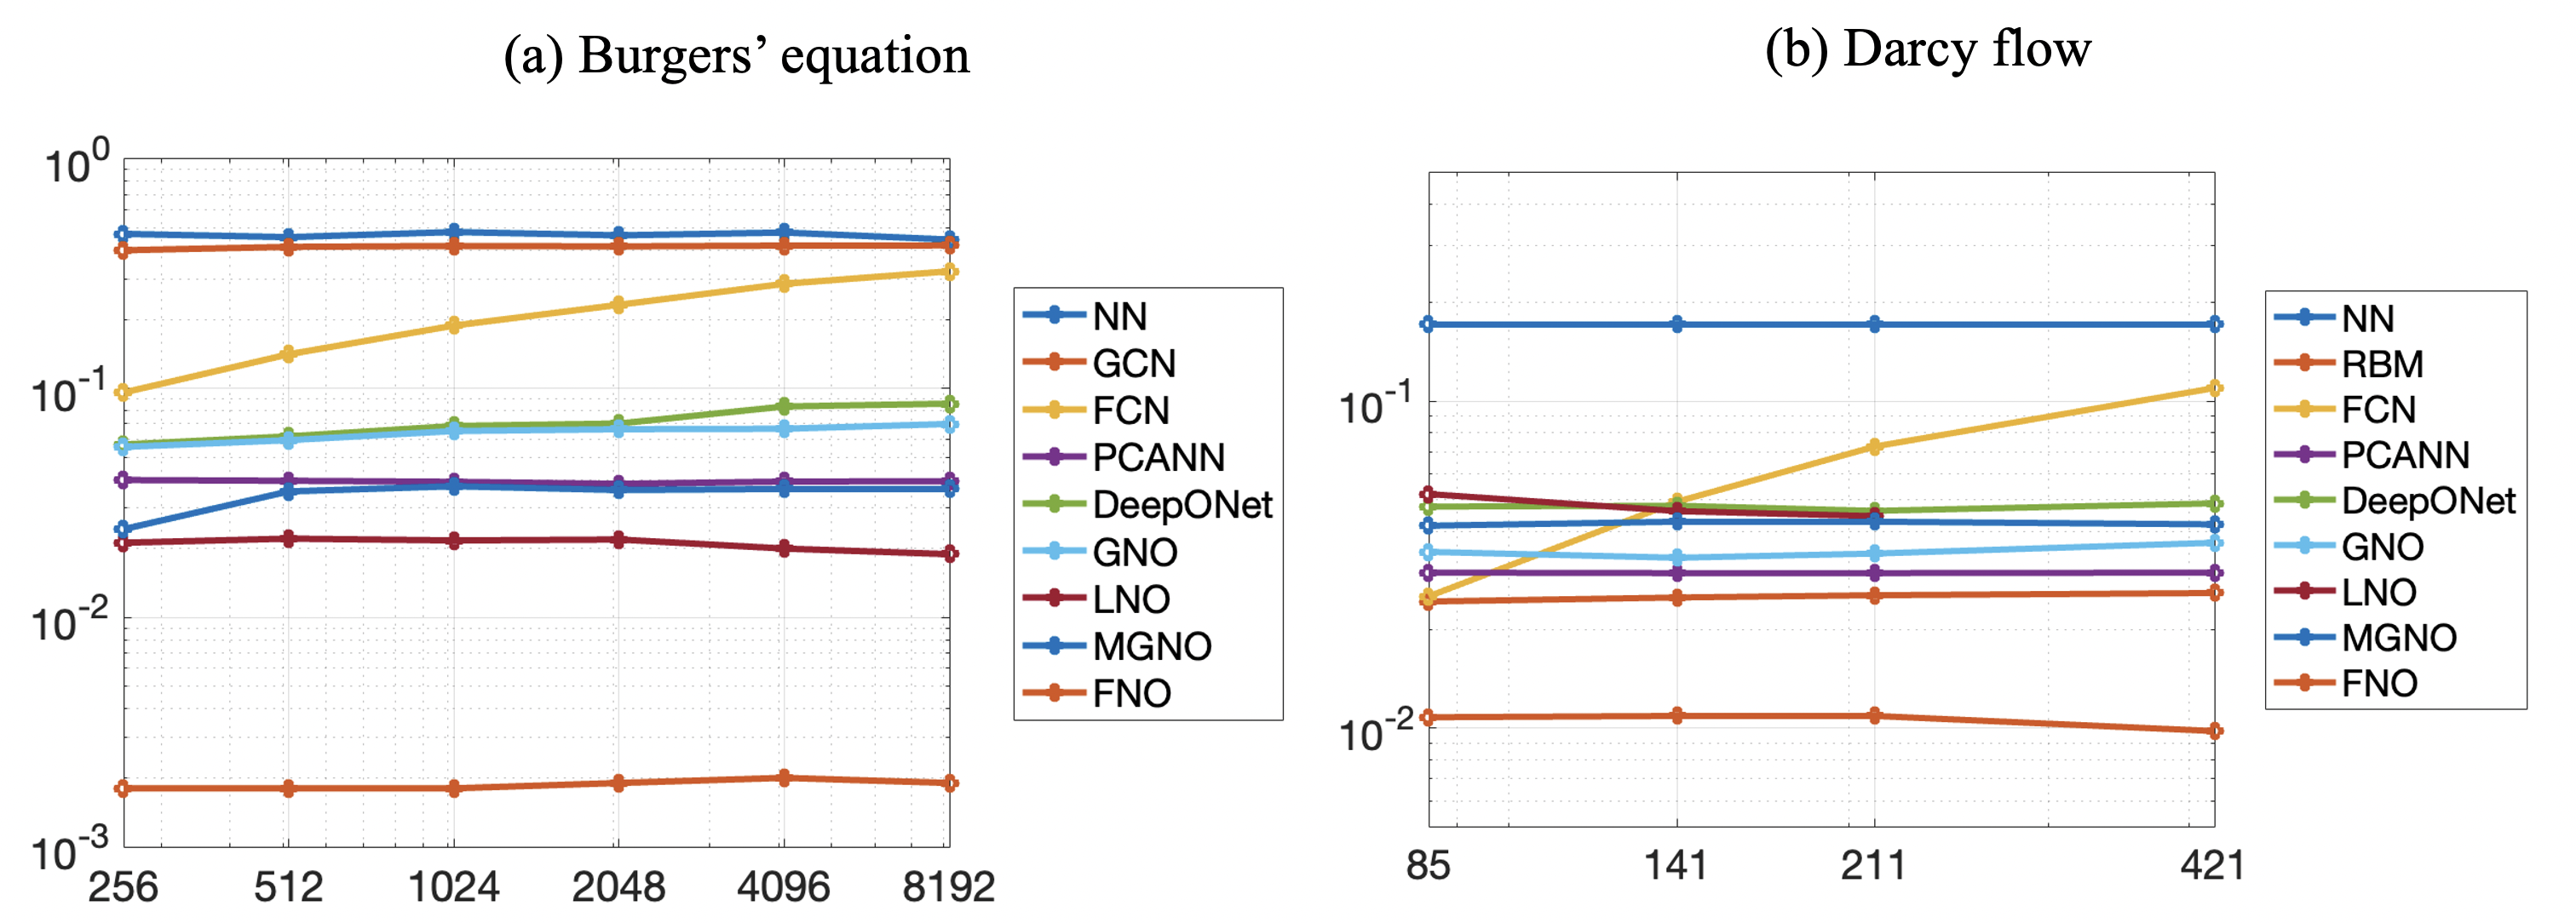
\includegraphics[width=\textwidth]{Figs/burger_darcy.png}
    \small{ \textbf{(a)} benchmarks on Burgers equation;  \textbf{(b)} benchmarks on Darcy Flow for different resolutions; Train and test on the same resolution.
    For acronyms, see Section \ref{sec:numerics}; details in Tables \ref{table:burgers}, \ref{table:darcy}.} 
    \caption{Benchmark on Burger's equation and Darcy Flow \done{It is confusing to have the two left hand panels with the right-most panel; the left most panels who resolution
    invariance very clear;y, the NSE panel is somewhat different. I suggest separate figures.}}
    \label{fig:error}
\end{figure}
\subsubsection{Darcy Flow}
\label{ssec:DF}

% {\bf The main points to get across here are (i) comparison of the
% approximation accuracy against other methods (standard NN,
% Zab, RBM); (ii) error as a function of resolution for different
% data set size; (iii) semi-supervised and mesh transference
% more generally; (iv) that low rank and/or multi-graph can make
% this competitive.}\\
The results of the experiments on Darcy flow are shown in Figure \ref{fig:error} and Table \ref{table:darcy}. All the methods, except for FCN, achieve invariance of
the error with respect to the resolution $s$. In the experiment, we tune each model across of range of different widths and depth to obtain
the choices used here; for DeepONet for example this leads to
8 layers and width 200 as reported above.

Within our hyperparameter search, the Fourier neural operator (FNO) obtains the lowest relative error. 
The Fourier based method likely sees this advantage because the output functions are smooth in these test problems.
We also note that is also possible to obtain better results on each model using modified architectures and problem specific feature engineering.
For example for DeepONet, using CNN on the branch net and PCA on the trunk net (the latter being similar to the method used in
\cite{Kovachki}) can achieve $0.0232$ relative $L_2$ error, as shown in \cite{lu2021comprehensive}, about half the size of the error we obtain here, but for a very coarse grid with $s=29.$
In the experiments the different approximation architectures are
such their training cost are similar across all the methods considered, for given $s.$ Noting this, and for example
comparing the graph-based neural operator methods such as GNO and MGNO that use Nystr\"om sampling in physical space with FNO, we
see that FNO is more accurate.
 
\begin{table}[ht]

\begin{center}
\begin{tabular}{l|llll}
\multicolumn{1}{c}{\bf Networks} 
&\multicolumn{1}{c}{\bf $s=85$}
&\multicolumn{1}{c}{\bf $s=141$} 
&\multicolumn{1}{c}{\bf $s=211$}
&\multicolumn{1}{c}{\bf $s=421$}\\
\hline
NN       &$0.1716$  &$0.1716$  &$0.1716$ &$0.1716$\\
FCN       &$0.0253$  &$0.0493$  &$0.0727$ & $0.1097$\\
PCANN      &$0.0299$  &$0.0298$  &$0.0298$ & $0.0299$\\
RBM    &$0.0244$ &$0.0251$ &$0.0255$ &$0.0259$ \\
DeepONet    &$0.0476$ &$0.0479$ &$0.0462$ &$0.0487$ \\
\hline 
GNO     &$0.0346$   &$0.0332$  &$0.0342$ &$0.0369$\\
LNO     &$0.0520$  &$0.0461$  &$0.0445$ &$-$\\
MGNO     &$0.0416$   &$0.0428$  &$0.0428$ &$0.0420$\\
FNO     &$\textbf{0.0108}$  &$\textbf{0.0109}$  &$\textbf{0.0109}$ &$\textbf{0.0098}$\\
\hline 
\end{tabular}
\end{center}
\caption{Relative error on 2-d Darcy Flow for different resolutions $s$.}
\label{table:darcy}
\end{table}

\subsubsection{Burgers' Equation}
\label{ssec:BE}

% {\bf The main points to get across here are: (i) that we can go beyond
% static elliptic problems (it still works hopefully using FFT
% architecture); (ii) that
% we can compose the solution operator and predict further in future
% than we train (generalization).}

The results of the experiments on Burgers' equation are shown in Figure \ref{fig:error} and Table \ref{table:burgers}. As for the Darcy problem, our instantiation of the Fourier neural operator obtains nearly one order of magnitude lower relative error compared to any benchmarks. The Fourier neural operator has standard deviation $0.0010$ and mean training error $0.0012$. If one replaces the ReLU activation by GeLU, the test error of the FNO is further reduced from $0.0018$ to \textbf{$0.0007$}.
We again observe the invariance of the error with respect to the resolution. 
It is possible to improve the performance on each model using modified architectures and problem specific feature engineering.
Similarly, the PCA-enhanced DeepONet with a proper scaling can achieve $0.0194$ relative $L_2$ error, as shown in \cite{lu2021comprehensive}, on a grid of resolution $s=128$.

\begin{table}[ht]

\begin{center}
\begin{tabular}{l|llllllll}
\multicolumn{1}{c}{\bf Networks}
&\multicolumn{1}{c}{\bf $s=256$}
&\multicolumn{1}{c}{\bf $s=512$}
&\multicolumn{1}{c}{\bf $s=1024$}
&\multicolumn{1}{c}{\bf $s=2048$} 
&\multicolumn{1}{c}{\bf $s=4096$}
&\multicolumn{1}{c}{\bf $s=8192$}\\
\hline 
NN       &$0.4714$ &$0.4561$
&$0.4803$ &$0.4645$ &$0.4779$ &$0.4452$ \\
GCN           &$0.3999$ &$0.4138$
&$0.4176$   &$0.4157$  &$0.4191$ &$0.4198$\\
FCN         &$0.0958$ &$0.1407$
&$0.1877$   &$0.2313$  &$0.2855$ &$0.3238$\\
PCANN       &$0.0398$ &$0.0395$
&$0.0391$   &$0.0383$  &$0.0392$ &$0.0393$\\
DeepONet       &$0.0569$ &$0.0617$
&$0.0685$   &$0.0702$  &$0.0833$ &$0.0857$\\
\hline 
GNO     &$0.0555$ &$0.0594$ &$0.0651$   &$0.0663$  &$0.0666$ &$0.0699$\\
LNO      &$0.0212$ &$0.0221$
   &$0.0217$  &$0.0219$ &$0.0200$ &$0.0189$\\
MGNO      &$0.0243$ &$0.0355$
   &$0.0374$  &$0.0360$ &$0.0364$ &$0.0364$\\
% FNO     &$\textbf{0.0149}$ &$\textbf{0.0158}$
%   &$\textbf{0.0160}$  &$\textbf{0.0146}$ &$\textbf{0.0142}$ &$\textbf{0.0139}$\\
FNO     &$\textbf{0.0018}$ &$\textbf{0.0018}$
   &$\textbf{0.0018}$  &$\textbf{0.0019}$ &$\textbf{0.0020}$ &$\textbf{0.0019}$\\
\hline 
\end{tabular}
\end{center}
\caption{ Relative errors on 1-d Burgers' equation for different resolutions $s$.} 
\label{table:burgers}
\end{table}





\begin{figure}[ht]
    \centering
    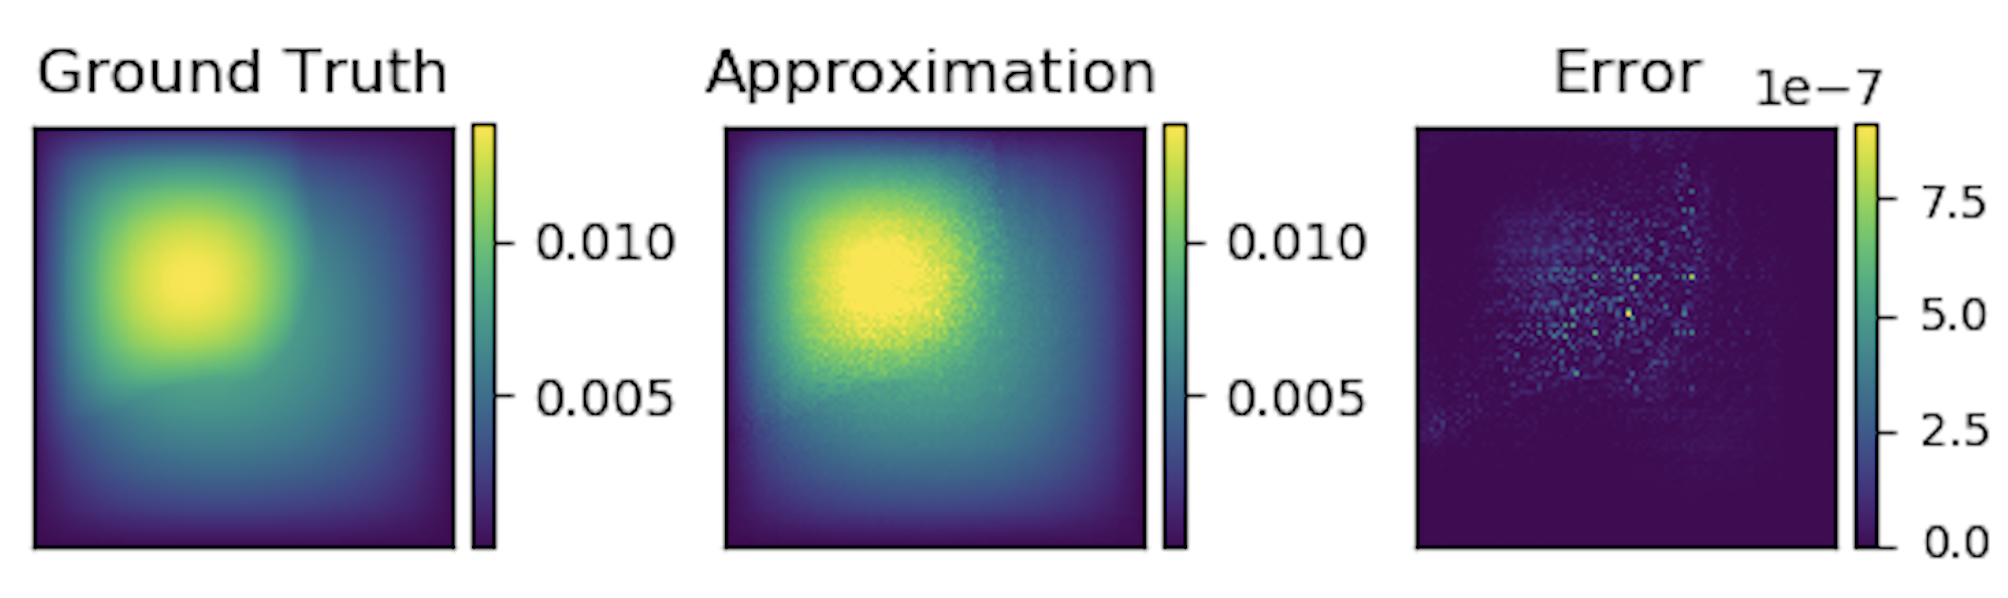
\includegraphics[width=\textwidth]{Figs/uai_16to241.png}
        \caption{Darcy, trained on $16 \times 16$, tested on $241 \times 241$}\label{fig:super1}
    \small{
    Graph kernel network for the solution of \eqref{ssec:darcy}. It can be trained on a small resolution and will generalize to a large one. The Error is point-wise absolute squared error.}
\end{figure}


\subsubsection{Zero-shot super-resolution.}
\label{sec:superresolution1}
The neural operator is mesh-invariant, so it can be trained on a lower resolution and evaluated at a higher resolution, without seeing any higher resolution data (zero-shot super-resolution).
Figure  \ref{fig:super1} shows an example of the Darcy Equation where we train the GNO model on $16 \times 16$ resolution data in the setting above and transfer to $256 \times 256$ resolution, demonstrating super-resolution in space.